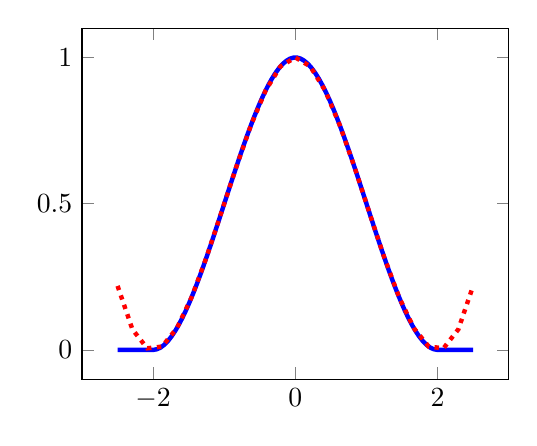
\begin{tikzpicture}
    \def\r(#1){abs(#1) / 2}%
    \begin{axis}
        \addplot[color=blue, ultra thick, samples=100, domain=-2.5:2.5]{
            \r(x) < 1 ? 2*(\r(x))^3-3*(\r(x))^2+1 : 0
        };
        \addplot[color=red, dotted, ultra thick, domain=-2.5:2.5]{
            2*(\r(x))^3-3*(\r(x))^2+1
        };
    \end{axis}
\end{tikzpicture}
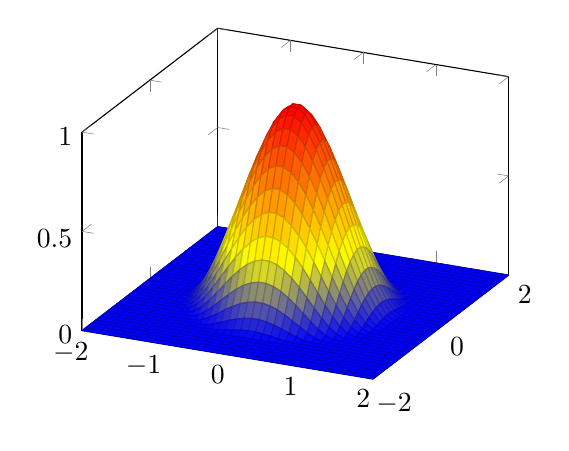
\begin{tikzpicture}[]
    \def\r(#1,#2){(((#1)^2 + (#2)^2) / 2)^0.5}%
    \def\K(#1,#2){2 * \r(#1,#2)^3 - 3 * \r(#1,#2)^2 + 1}
    \begin{axis}[
        % xmin=-2.5,xmax=2,
        % ymin=-2.5,ymax=2,
        zmin= 0  ,zmax=1,
        % axis line style={draw=none},
        % axis equal image,
    ]
    \addplot3[
        surf,
        domain=-2:2,
        samples=40
    ]
    % K(x,y) = 2r^3 - 3r^2 + 1 if r < 1 else 0
    % r = sqrt(x^2 + y^2) / R
    % R = desired radius, lets use 2
    % therefore we get:
    % r = sqrt(x^2 + y^2) / 2
    % K(x,y) = sqrt(x^2 + y^2) / 2 < 1 ? 2 * (sqrt(x^2 + y^2) / 2) ^ 3 - 3 * (sqrt(x^2 + y^2) / 2) ^ 2 + 1 : 0
    {\r(x,y) < 1 ? \K(x,y) : 0};% < 1 ? 2 * r(x,y) ^ 3 - 3 * r(x,y) ^ 2 + 1 : 0};
    \end{axis}
\end{tikzpicture}
\pgfplotsset{width=7cm,compat=1.8}
\pgfmathdeclarefunction{gauss}{2}{%
    \pgfmathparse{1/(#2*sqrt(2*pi))*exp(-((x-#1)^2)/(2*#2^2))}%
}
\begin{tikzpicture}
    \begin{axis}[every axis plot post/.append style={
        ultra thick, samples=100, domain=-2.5:2.5, mark=none}]
        \addplot {abs(x) < 2 ? 1.6 * gauss(0,2/3) : 0};
    \end{axis}
\end{tikzpicture}
\begin{tikzpicture}
    \begin{axis}[every axis plot post/.append style={
        ultra thick, samples=100, domain=-12:12, mark=none}]
        \addplot {abs(x) < 10 ? 8.4 * gauss(0,10/3) : 0};
        \def\r(#1){abs(#1) / 10}%
        \addplot[color=red, dotted, ultra thick, samples=100, domain=-12:12]{
            \r(x) < 10 ? 2*(\r(x))^3-3*(\r(x))^2+1 : 0
        };
    \end{axis}
\end{tikzpicture}